\subsection{Round 1 Solutions}\label{S::2024-J-1}

\begin{resources}
    Review by \resit{https://www.youtube.com/watch?v=nSo2yddsjrk}{Way Tan}
\end{resources}

\begin{question}[D]\label{Q::2024-J-1-1}
    If $x^2 + 4x + 16 = 0$, what is the value of $x^3$?
    \begin{tasks}(5)
        \task 4
        \task 8
        \task 16
        \task 64
        \task 128
    \end{tasks}
\end{question}
\begin{solution*}
    By the quadratic formula, we have \[x = -2 + 2\sqrt3 i = 4\bp{-\frac12 \pm \frac{\sqrt3}{2} i} = 4e^{\pm\frac{2\pi}{3} i}.\] Thus, $x^3 = 4^3 e^{\pm 2\pi i} = 64$.
\end{solution*}

\begin{question}[D]\label{Q::2024-J-1-2}
    Let $a$ be a real number that satisfies $-1 < a < 0$. Which of the following is true?
    \begin{tasks}(5)
        \task! $\pi^a < \frac1\pi < (\frac1\pi)^a$
        \task! $\pi^a < (\frac1\pi)^a < \frac1\pi$
        \task! $\frac1\pi < (\frac1\pi)^a < \pi^a$
        \task! $\frac1\pi < \pi^a < (\frac1\pi)^a$
        \task! $(\frac1\pi)^a < \pi^a < \frac1\pi$
    \end{tasks}
\end{question}
\begin{solution*}
    We are tasked with ordering $\pi^{-1}$, $\pi^{a}$ and $\pi^{-a}$. This is equivalent to ordering $-1$, $a$ and $-a$. Since $-1 < a < 0$, we clearly have $-1 < a < -a$. Thus, $\pi^{-1} < \pi^a < \pi^{-a}$.
\end{solution*}

\begin{question}[B]\label{Q::2024-J-1-3}
    How many non-congruent triangles are there whose sides have integer lengths and the longest side has length 10 units?
    \begin{tasks}(5)
        \task 25
        \task 30
        \task 35
        \task 40
        \task 45
    \end{tasks}
\end{question}
\begin{solution*}
    Let $a$ and $b$ be the lengths of the legs of the triangle. By the triangle inequality, we must have $a + b > 10$. Without loss of generality, let $1 \leq a \leq b \leq 10$. Let $a$ be fixed. Then $b \in \bc{\max{11-a, a}, \ldots, 10}$. This gives $\min{a, 11-a}$ possible values of $b$. Summing from $a = 1$ to $a = 10$, we have 30 possible pairs of side lengths and hence 30 possible triangles, which are guaranteed to be non-congruent by construction.
\end{solution*}

\begin{question}[C]\label{Q::2024-J-1-4}
    In the diagram below, the points $B$ and $E$ lie on $AF$ and $DF$ respectively, and $AE$ and $BD$ intersect at $C$. If $AB = AC$, $BD = BF$ and $EA = EF$, find $\angle BAC$.
    \begin{center}
        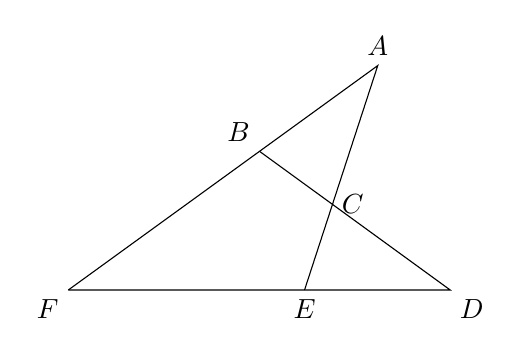
\begin{tikzpicture}
            \coordinate[label=above:$A$] (A) at (3.93, 2.85);
            \coordinate[label=above left:$B$] (B) at (2.43, 1.76);
            \coordinate[label=right:$C$] (C) at (3.35, 1.09);
            \coordinate[label=below right:$D$] (D) at (4.85, 0);
            \coordinate[label=below:$E$] (E) at (3, 0);
            \coordinate[label=below left:$F$] (F) at (0, 0);

            \draw (F) -- (A) -- (E);
            \draw (B) -- (D) -- (F);
        \end{tikzpicture}
    \end{center}
    \begin{tasks}(5)
        \task $30\deg$
        \task $33\deg$
        \task $36\deg$
        \task $38\deg$
        \task $40\deg$
    \end{tasks}
\end{question}
\begin{solution*}
    Let $\angle BAC = \a$. Since $\triangle FEA$ is isosceles, we have $\angle BFD = \a$. Since $\triangle FBD$ is isosceles, we also have $\angle BDF$. Thus, $\angle FBD = 180\deg - 2\a$. Meanwhile, because $\triangle BAC$ is isosceles, $\angle ABC = 90\deg - \frac12 \a$. Hence, \[\angle FBD + \angle ABD = 180\deg \implies \bp{180\deg - 2\a} + \bp{90\deg - \frac12 \a} = 180\deg \implies \a = 36\deg.\]
\end{solution*}

\begin{question}[C]\label{Q::2024-J-1-5}
    Let $x$, $y$ and $z$ be real numbers such that $x \neq 0$, $y - z \neq 0$ and $z + x \neq 0$. If $\dfrac{2}{x} = \dfrac{4}{y - z} = \dfrac{5}{z + x}$, find the value of $\dfrac{7x-y}{y+2z}$.
    \begin{tasks}(5)
        \task $\dfrac{11}{17}$
        \task $-\dfrac{11}{17}$
        \task $\dfrac{7}{13}$
        \task $-\dfrac{7}{13}$
        \task 1
    \end{tasks}
\end{question}
\begin{solution*}
    Taking reciprocals, we have \[\frac{x}{2} = \frac{y-z}{4} = \frac{z+x}{5} \implies y = \frac72 x, \quad z = \frac32 x.\] Hence, \[\frac{7x - y}{y + 2x} = \frac{7x - \frac72 x}{\frac72 x + 2(\frac32 x)} = \frac{7}{13}.\]
\end{solution*}

\begin{question}[76]\label{Q::2024-J-1-6}
    Let $N$ be a 2-digit whole number. When 2692 is divided by $N$, the remainder is 13, and when 2978 is divided by $N$, the remainder is 14. Find the sum of all the possible values of $N$.
\end{question}
\begin{solution*}
    We are given that $2692 \equiv 13 \pmod{N}$ and $2978 \equiv 14 \pmod{N}$. Thus, \[2679 \equiv 2964 \equiv 0 \pmod{N} \implies 285 = 2964 - 2679 \equiv 0 \pmod{N}.\] Since $285 = 3 \cdot 5 \cdot 19$, the only two-digit factors of 285 are 15, 19, 57, 95. However, $N$ clearly cannot end in 5. Thus, $N$ can only be 19 or 57. Testing these two values, we see that they indeed satisfy the given conditions. Thus, the sum of all the possible values of $N$ is $19 + 57 = 76$.
\end{solution*}

\begin{question}[89]\label{Q::2024-J-1-7}
    If $x$ is a positive integer such that $2^x + 2^{89} = 512^{10}$, find the value of $x$.
\end{question}
\begin{solution*}
    Note that $512 = 2^{9}$. We hence have $2^x = 2^{90} - 2^{89} = 2^{89}$, whence $x = 89$.
\end{solution*}

\begin{question}[17]\label{Q::2024-J-1-8}
    The diagram shows a right-angled triangle $ABC$. The sides $AC$ and $AB$ are in the ratio $3:5$. The point $D$ lies on $BC$ such that $AD$ is perpendicular to $BC$. Furthermore, $DB$ is 8 cm longer than $CD$. What is the length of $BC$ in cm?
    
    \begin{center}
        \begin{tikzpicture}[scale=0.4]
            \coordinate[label=below left:$A$] (A) at (0, 0);
            \coordinate[label=below right:$B$] (B) at (14.577, 0);
            \coordinate[label=above left:$C$] (C) at (0, 8.746);
            \coordinate[label=above right:$D$] (D) at (3.858, 6.43);

            \draw (A) -- (B) -- (C) -- (A) -- (D);

            \draw pic [draw, angle radius=2mm] {right angle = C--A--B};
            \fill (D) circle[radius=5pt];
        \end{tikzpicture}
    \end{center}
\end{question}
\begin{solution*}
    Let $AC = 3x$ and $CD = y$. Then $AB = 5x$ and $DB = y + 8$. By the geometric mean theorem, we have \[BD \cdot DC = AD^2 \implies y(y+8) = AD^2. \tag{1}\] Applying Pythagoras' theorem to $\triangle ABC$ and $\triangle ADC$, we see that \[AB^2 + AC^2 = BC^2 \implies 34x^2 = (2y + 8)^2\] and \[AD^2 + DC^2 = AC^2 \implies AD^2 = 9x^2 - y = \frac{9}{34}(2y + 8)^2 - y^2. \tag{2}\] Equating (1) and (2), we see that \[y(y + 8) = \frac{9}{34}(2y + 8)^2 - y^2,\] which gives $y = \frac92$, whence $BC = 2y + 8 = 17$.
\end{solution*}

\begin{question}[1825]\label{Q::2024-J-1-9}
    Let $n$ be a positive integer. Suppose that $a_1, a_2, a_3, \ldots$ is a sequence of numbers defined by \[a_1 = \sqrt{(n+3)(n-1) + 4}, \quad a_k = \sqrt{(n + 2k + 1)a_{k-1} + 4} \quad \text{for $k \geq 2$}.\] If $a_{100} = 2024$, find the value of $n$.
\end{question}
\begin{solution*}
    We claim that $a_k = n + 2k - 1$ for $k \geq 2$. Consider the base case $k = 1$: Observe $(n + 3)(n - 1) + 4 = \bs{(n+1) + 2}\bs{(n + 1) - 2} + 4 = (n+1)^2$. Hence, $a_1 = n + 1$. Now suppose that $a_m = n + 2m - 1$ for some positive integer $m$. Observe that
    \begin{align*}
        a_{m + 1} &= \sqrt{(n + 2(m + 1) + 1)a_{m} + 4} = \sqrt{(n + 2m + 1 + 2)(n + 2m + 1 - 2) + 4}\\
        &= \sqrt{(n + 2m + 1)^2 - 2^2 + 4} = \sqrt{(n + 2m + 1)^2} = n + 2m + 1 = n + 2(m + 1) - 1.
    \end{align*}
    This closes the induction. We hence see that $a_{100} = n + 200 - 1 = 2024$, whence $n = 1825$.
\end{solution*}

\begin{question}[10]\label{Q::2024-J-1-10}
    Let $N$ be the smallest positive integer such that the sum of its digits is 2024. What is the sum of the digits of the number $N + 2$.
\end{question}
\begin{solution*}
    Since $N$ is minimal, it must be of the form $\ol{a9\cdots9}$, where $a$ is an integer between 1 and 9. This gives $a + 9 + \cdots + 9 = 2024$. Reducing modulo 9 yields $a = 8$. Thus, $N = \ol{89\cdots9}$, whence $N + 2 = \ol{90\cdots1}$. The digit sum of $N + 2$ is hence $9 + 1 = 10$.
\end{solution*}

\begin{question}[19]\label{Q::2024-J-1-11}
    If $a$ and $b$ are non-zero real numbers such that $\dfrac1b - \dfrac1a = 4$, find the value of $\dfrac{3a + 7ab - 3b}{a - 3ab - b}$.
\end{question}
\begin{solution*}
    Multiplying through by $ab$ yields \[a - b = 4ab \implies ab = \frac{a-b}{4}.\] Thus, \[\frac{3a + 7ab - 3b}{a - 3ab - b} = \frac{(3a - 9ab - 3b) + 16ab}{a - 3ab - b} = 3 + \frac{4(a-b)}{a - 3(\frac{a-b}{4}) - b} = 3 + \frac{4}{1 - \frac34} = 19.\]
\end{solution*}

\begin{question}[5]\label{Q::2024-J-1-12}
    If the 5-digit whole number $\ol{11ab6}$ is a perfect square, find the value of $a + b$.
\end{question}
\begin{solution*}
    Let $\ol{11ab6} = m^2$. Then $10000 < m^2 < 12000$, whence $100 < m < 109$. Also note that the ones digit of $m$ is either 4 or 6. We hence have $m = 104$ or $m = 106$. Testing both cases, we see that $104^2 = 10816$ while $106^2 = 11236$, whence $a + b = 2 + 3 = 5$.
\end{solution*}

\begin{question}[9920]\label{Q::2024-J-1-13}
    Let $N = 1 \times 2 + 2 \times 3 + 3 \times 4 + \cdots + 30 \times 31$. Find the value of $N$.
\end{question}
\begin{solution*}
    Clearly, \[N = \sum_{i = 1}^{30} i(i + 1) = \sum_{i = 1}^{30} \bp{i^2 + i}.\] Using the standard formulae for power sums, we end up with \[N = \frac{30(30 + 1)(2 \cdot 30 + 1)}{6} + \frac{30(30 + 1)}{2} = 9920.\]
\end{solution*}

\clearpage
\begin{question}[23]\label{Q::2024-J-1-14}
    Let $x$ and $y$ be non-zero real numbers where $x \neq y$. If $x^2 + \sqrt3 y = 4$ and $y^2 + \sqrt3 x = 4$, find the value of $\bp{\dfrac{y}{x}}^2 + \bp{\dfrac{x}{y}}^2$.
\end{question}
\begin{solution*}
    Let $x \mapsto \sqrt3 x$ and $y \mapsto \sqrt 3 y$, which  obviously do not affect the value of $(\frac{y}{x})^2 + (\frac{x}{y})^2$. The given equations simplify to $3x^2 + 3y = 4$ and $3y^2 + 3x = 4$. 
    
    Summing the two equations together and completing the square, we have \[\bp{x + \frac12}^2 + \bp{y + \frac12}^2 = \frac{19}{6}.\] Observe that this describes a circle symmetric about the line $y = x$. Subtracting the two equations and completing the square, we have \[\bp{x - \frac12}^2 = \bp{y - \frac12}^2.\]  Combining this with the symmetry of $(x, y)$ about $y = x$, it follows that $(x, y)$ lies on the line $y = -x + 1$. Hence, \[-x + 1 = \frac{4 - 3x^2}{3} \implies x,y = \frac{3 \pm \sqrt{21}}{6},\] where $x$ and $y$ take different branches of the square root. Thus, \[\bp{\frac{y}{x}}^2 + \bp{\frac{x}{y}}^2 = \frac{x^4 + y^4}{(xy)^2} = \frac{\bp{3 + \sqrt{21}}^4 + \bp{3 - \sqrt{21}}^4}{\bs{\bp{3 + \sqrt{21}}\bp{3 - \sqrt{21}}}^2} = 23.\]
\end{solution*}

\begin{question}[72]\label{Q::2024-J-1-15}
    Find the sum of all 2-digit even numbers $N$ with the following property: $N$ is a multiple of the product of its two digits.
\end{question}
\begin{solution*}
    Let $N = 10a + b$, where $a$ and $b$ are integers such that $1 \leq a \leq 9$ and $b \in \bc{0, 2, 4, 6, 8}$. The given condition translates to $10a + b = kab$, where $k$ is a positive integer. Let $b = 2b'$, where $b' \in \bc{0, 1, \ldots, 4}$. Then $(kb' - 5)a = b'$.

    \case{1} Suppose $b' = 0$. Then $a = 0$, a contradiction.
    
    \case{2} Suppose $b' = 1$. Then $(k-5)a = 1$, whence $a$ can only be 1 (when $k = 6$). Hence, $N = 12$ is a solution.
    
    \case{3} Suppose $b' = 2$. Then $(2k-5)a = 2$. Then $a$ can only be 2 (when $k = 3$). Hence, $N = 24$ is a solution.

    \case{4} Suppose $b' = 3$. Then $(3k - 5)a = 3$. Then $a$ can only be 3 (when $k = 2$). Hence, $N = 36$ is a solution.

    \case{5} Suppose $b' = 4$. Then $(4k - 5)a = 4$. Since $4k - 5 \neq 1, 2, 4$, there are no solutions in this case.

    Thus, the only possible values of $N$ are 12, 24 and 36. The desired answer is hence $12 + 24 + 36 = 72$.
\end{solution*}

\begin{question}[25]\label{Q::2024-J-1-16}
    In the diagram below, $AEB$ is an isosceles right-angled triangle and $ABG$ is a $30\deg$-$60\deg$-$90\deg$ right-angled triangle with $\angle GAB = 30\deg$. The sides $AG$ and $BE$ intersect at $H$. If the area of triangle $AHE$ is 50 cm$^2$, find the area of triangle $BGH$ in cm$^2$.

    \begin{center}
        \begin{tikzpicture}
            \coordinate[label=below left:$A$] (A) at (-4, 0);
            \coordinate[label=below right:$B$] (B) at (4, 0);
            \coordinate[label=above:$E$] (E) at (0, 4);
            \coordinate[label=above:$G$] (G) at (2, 3.464);
            \coordinate[label=above:$H$] (H) at (1.072, 2.928);

            \draw (A) -- (B) -- (E) -- (A);
            \draw (A) -- (G) -- (B);

            \tkzMarkSegment[pos=.5,mark=|](A,E);
            \tkzMarkSegment[pos=.5,mark=|](B,E);

            \draw pic [draw, angle radius=2mm, ""] {right angle = A--E--B};
            \draw pic [draw, angle radius=2mm, ""] {right angle = A--G--B};
        \end{tikzpicture}
    \end{center}
\end{question}
\begin{solution*}
    Observe that $ABGE$ is cyclic, where $AB$ is the diameter of $(ABGE)$. Let $\a = \angle EAB$. Then $\angle EBA = \a$. Thus, $\angle EAH = \a - 30\deg$ and $\angle GBH = 60\deg - \a$. Since $\angle EAH = \angle GBH$, we obtain $\a = 45\deg$. We thus have $AE = \sqrt2 r$, where $r = \frac12 AB$ is the radius of $(ABGE)$. Also, $GB = AB \sin 30\deg = r$. Since $\triangle AEH$ and $\triangle BGH$ are similar, we see that \[\frac{HB}{GB} = \frac{HA}{EA} \implies \frac{HB}{EH} = \frac1{\sqrt2}.\] The ratio of similarity is thus $\frac1{\sqrt2}$, whence $[BGH] = \bp{\frac1{\sqrt2}}^2 [AEH] = 25$ cm$^2$.
\end{solution*}

\begin{question}[2451]\label{Q::2024-J-1-17}
    Find the smallest positive integer $n$ such that $\sqrt{n} - \sqrt{n - 1} < \dfrac1{99}$.
\end{question}
\begin{solution*}
    Squaring the inequality, we see that \[2\sqrt{n(n-1)} > 2n - 1 - 99^{-2}.\] Squaring once more, we obtain \[1 + (2 - 4n)99^{-2} + 99^{-4} < 0.\] Rearranging, we obtain \[n > \frac{99^2 + 99^{-2} + 2}{4} \approx 2450.75,\] whence $\min n = 2451$.
\end{solution*}

\begin{question}[32]\label{Q::2024-J-1-18}
    Let $a$, $b$ and $c$ be real numbers such that $a + b + c = 8$ and $ab + bc + ca = 0$. Find the maximum value of $3(a + b)$.
\end{question}
\begin{solution*}
    From the second equation, we have $c = -\frac{ab}{a + b}$. Substituting this into the first equation and clearing denominators yields \[(a+b)^2 - 8(a+b) - ab = 0.\] By the AM-GM inequality, we have $ab \leq \frac14 (a+b)^2$. Hence, \[(a+b)^2 - 8(a+b) - \frac14(a+b) \leq 0 \implies 3(a+b)^2 - 32(a+b) \leq 0.\] Thus, $\max (a+b) = \frac{32}{3}$, whence $\max 3(a+b) = 32$.
\end{solution*}

\begin{question}[16]\label{Q::2024-J-1-19}
    In the table below, every row and column is an infinite arithmetic progression.

    \begin{table}[H]
        \centering
        \begin{tabular}{|c|c|c|c|c|c|}
        \hline
        1 & 3 & 5 & 7 & 9 & $\cdots$ \\\hline
        3 & 6 & 9 & 12 & 15 & $\cdots$ \\\hline
        5 & 9 & 13 & 17 & 21 & $\cdots$ \\\hline
        7 & 12 & 17 & 22 & 27 & $\cdots$ \\\hline
        9 & 15 & 21 & 27 & 33 & $\cdots$ \\\hline
        $\vdots$ & $\vdots$ & $\vdots$ & $\vdots$ & $\vdots$ & $\cdots$\\\hline
        \end{tabular}
    \end{table}

    How many times does the number 2025 appear in the table?
\end{question}
\begin{solution*}
    Let $a_{ij}$ be the number in the $i$th row and $j$th column of the table, where $i, j > 0$. Observe that $a_{i+1,j} - a_{ij} = j+1$. Since $a_{1j} = 2j - 1$, it follows that \[a_{ij} = 2j - 1 + (i-1)(j+1) = (i+1)(j+1) - 3.\] Consider $a_{ij} = 2025$. Then $(i + 1)(j + 1) = 2028 = 2^2 \cdot 3 \cdot 13^2$. The number of possible pairs of $(i, j)$ is thus the number of positive pairs of factors of 2028 (excluding 1). This gives a total of $3 \cdot 2 \cdot 3 - 2 = 16$ possibilities. Note that we subtract 2 as we need to exclude $(1, 2028)$ and $(2028, 1)$.
\end{solution*}

\begin{question}[3]\label{Q::2024-J-1-20}
    In the diagram below, $ABC$ is a right-angled triangle. Points $D$ and $E$ lie on $AB$ while points $F$ and $G$ lie on $BC$ such that $\triangle EFG$ and $\triangle DGC$ are right-angled isosceles triangles. It is given that $DC = 3EG$ and the area of $\triangle DGC = 1$ cm$^2$. What is the area of $\triangle ADC$ in cm$^2$?

    \begin{center}
        \begin{tikzpicture}[scale=0.5]
            \coordinate[label=above:$A$] (A) at (4, 9);
            \coordinate[label=below left:$B$] (B) at (-0.5, 0);
            \coordinate[label=below right:$C$] (C) at (4, 0);
            \coordinate[label=above left:$D$] (D) at (1,3);
            \coordinate[label=above left:$E$] (E) at (0, 1);
            \coordinate[label=below:$F$] (F) at (0, 0);
            \coordinate[label=below:$G$] (G) at (1, 0);
    
            \draw (A) -- (B) -- (C) -- (A);
            \draw (F) -- (E) -- (G) -- (D) -- (C);

            \draw pic [draw, angle radius=1.5mm] {right angle = E--F--G};
            \draw pic [draw, angle radius=1.5mm] {right angle = D--G--C};
        \end{tikzpicture}
    \end{center}
\end{question}
\begin{solution*}
    Since $\triangle EFG$ and $\triangle DGC$ are similar, we get $\frac{EF}{DG} = \frac{EG}{DC} = \frac13$. Since $\triangle DEG$ and $\triangle FEG$ have the same height ($FG$), we get \[[DEG] = 3 \, [FEG] = 3 \cdot \bp{\frac13}^2 = \frac13.\] Observe that $\triangle DEG$ and $\triangle ADC$ are also similar. Since $\frac{DC}{EG} = 3$, we obtain \[[ADC] = 3^2 \, [DEG] = 3.\]
\end{solution*}

\begin{question}[504]\label{Q::2024-J-1-21}
    How many different 4-tuples ($a$, $b$, $c$, $d$) are there, where $a$, $b$, $c$ and $d$ are positive integers, such that \[a > b > c > d, \quad a + b + c + d = 2024 \quad \text{and} \quad a^2 - b^2 + c^2 - d^2 = 2024?\]
\end{question}
\begin{solution*}
    Observe that \[a^2 - b^2 + c^2 - d^2 = a + b + c + d \implies (a-b-1)(a+b) + (c-d-1)(c+d) = 0.\] Since $a+b$ and $c+d$ are positive, it must be that one of $a-b-1$ and $c-d-1$ is negative, or both are zero.
    
    \case{1} Suppose $a - b - 1 < 0$. Then $a - b < 1$. However, since $a > b$, we know that $a - b > 0$, a contradiction. A similar argument holds for the case where $c - d - 1 < 0$.

    \case{2} Suppose $a - b - 1 = 0$ and $c - d - 1 = 0$. Then $a = b+1$ and $c = d + 1$. Substituting this into the two equations, we see that \[b + d = 1011.\] Observe that $b \geq d + 2$, whence \[b + (d+2) = 1013 \implies b \geq 507\] Additionally, $\max b$ occurs when $d = 1$ and $c = 2$, thus \[(\max b + 1) + \max b + 2 + 1 = 2024 \implies \max b = 1010.\] There are hence $1010-507+1 = 504$ possible values for $b$, giving a total of 504 different 4-tuples.
\end{solution*}

\begin{question}[360]\label{Q::2024-J-1-22}
    Points $A$ and $B$ lie on the graph of $y = x^2 + 5x - 8$ such that $A$, $B$ and the origin $O$ are collinear and $\abs{OB} = 2\abs{OA}$. It is given that $A$ lies in the first quadrant. Find $\abs{AB}^2$.
\end{question}
\begin{solution*}
    We have that $A$ and $B$ are the intersections between $y = x^2 + 5x - 8$ and $y = kx$, where $k > 0$. Solving the two equations simultaneously, we end up with $A(x_A, kx_A)$ and $B(x_B, kx_B)$, where \[x_A = \frac{k-5 + \sqrt{k^2 - 10k + 57}}{2}, \qquad x_B = \frac{k-5 - \sqrt{k^2 - 10k + 57}}{2}.\] Since $\abs{OB} = 2\abs{OA}$, we get \[x_B^2 + k^2x_B^2 = 4x_A^2 + 4k^2 x_A^2 \implies \bp{k^2 - 1}\bp{4x_A^2 - x_B^2} = 0.\] Clearly $k \neq 1$. Hence, we have $4x_A^2 - x_B^2 = (2x_A - x_B)(2x_A + x_B) = 0$. Since $\abs{x_A} < \abs{x_B}$, we have $2x_A + x_B = 0$. This gives \[2\bp{k-5 + \sqrt{k^2 - 10k + 57}} + \bp{k-5 - \sqrt{k^2 - 10k + 57}} = 0,\] which implies that \[3(k - 5) + \sqrt{k^2 - 10k + 57} = 0 \implies \sqrt{k^2 - 10k + 57} = 3(5 - k).\] Squaring, we get \[k^2 - 10k + 57 = 225 - 90k + 9k^2 \implies k^2 - 10k + 21 = 0,\] whence $k = 3$ or $k = 7$. Testing these two values, we see that only $k = 3$ satisfies the condition $\abs{OB} = 2\abs{OA}$, where $\abs{OA} = \sqrt{40}$ and $\abs{OB} = \sqrt{160}$, thus $\abs{AB}^2 = (3\sqrt{40})^2 = 360$.
\end{solution*}

\begin{question}[15630]\label{Q::2024-J-1-23}
    The diagram below shows a regular hexagon that is divided into six congruent triangular regions $A$, $B$, $C$, $D$, $E$ and $F$. Two triangular regions are adjacent if they share a common side. For example, $A$ and $B$ are adjacent but $A$ and $C$ are not adjacent. In how many ways can we colour these regions $A$, $B$, $C$, $D$, $E$ and $F$ using six different colours such that the adjacent regions do not receive the same colour? (Note that not all six colours need to be used in colouring the six regions and non-adjacent regions can receive the same colour).

    \begin{center}
        \begin{tikzpicture}[scale=1.5]
            \coordinate (A) at (1, 0);
            \coordinate (B) at (0.5, 0.866);
            \coordinate (C) at (-0.5, 0.866);
            \coordinate (D) at (-1, 0);
            \coordinate (E) at (-0.5, -0.866);
            \coordinate (F) at (0.5, -0.866);
            \coordinate (O) at (0, 0);

            \draw (A) -- (B) -- (C) -- (D) -- (E) -- (F) -- (A);
            \draw (C) -- (F);
            \draw (B) -- (E);
            \draw (A) -- (D);

            \node at ($(A)!0.5!(B)!0.3!(O)$) {C};
            \node at ($(B)!0.5!(C)!0.3!(O)$) {B};
            \node at ($(C)!0.5!(D)!0.3!(O)$) {A};
            \node at ($(D)!0.5!(E)!0.3!(O)$) {F};
            \node at ($(E)!0.5!(F)!0.3!(O)$) {E};
            \node at ($(F)!0.5!(A)!0.3!(O)$) {D};
        \end{tikzpicture}
    \end{center}
\end{question}
\begin{solution*}
    Let $A_k$ be the event that at least $k$ pairs of adjacent regions have the same colour. By the inclusion-exclusion principle, the number of colourings such that no two pairs have the same colour is given by \[\abs{A_0} - \abs{A_1} + \abs{A_2} - \abs{A_3} + \abs{A_4} - \abs{A_5} + \abs{A_6}.\] Now observe that for $0 \leq k \leq 5$, we have \[\abs{A_k} = \binom{6}{k} 6^{6-k}:\] $\binom{6}{k}$ ways to choose the $k$ pairs, and $6^{6-k}$ ways to colour the $6-k$ groups of regions (where we group a pair of regions together). Meanwhile, for $k = 6$, we obviously have \[\abs{A_6} = 6.\] Thus, the desired answer is \[\sum_{k = 0}^5 \binom{6}{k} (-1)^k 6^{n-k} + 6 = (6-1)^6 + (6-1) = 15630.\]
    \begin{remark}
        In general, the number of ways to colour a cycle graph with $n$ nodes ($C_n$) with $\l$ colours is given by $(\l - 1)^n + (-1)^n (\l - 1)$. This is called the chromatic polynomial of $C_n$. In our case, we have $n = \l = 6$.
    \end{remark}
\end{solution*}

\begin{question}[45]\label{Q::2024-J-1-24}
    The diagram below shows three toy cars moving in a rectangular circuit $ABCD$ where $AB = 10$m and $BC = 20$m. Toy cars $M$ and $N$ start from the vertices $A$ and $C$ respectively and move in an anti-clockwise direction with constant speeds 10 m/min and 4 m/min respectively. Toy car $P$ starts from $C$ and moves in a clockwise direction with a constant speed of 8 m/min.
    \begin{center}
        \begin{tikzpicture}
            \coordinate[label=above left:$A$] (A) at (0, 4);
            \coordinate[label=above right:$D$] (B) at (8, 4);
            \coordinate[label=below right:$C$] (C) at (8, 0);
            \coordinate[label=below left:$B$] (D) at (0, 0);
            \coordinate[label=left:$M$] (M) at (0, 3);
            \coordinate[label=right:$N$] (N) at (8, 1);
            \coordinate[label=below:$P$] (P) at (7, 0);
    
            \draw (A) -- (B) -- (C) -- (D) -- (A);
        
            \draw[very thick, ->] (0.25, 3) -- (0.25, 2);
            \draw[very thick, ->] (7, 0.25) -- (6, 0.25);
            \draw[very thick, ->] (7.75, 1) -- (7.75, 2);

            \fill (M) circle[radius=2.5pt];
            \fill (N) circle[radius=2.5pt];
            \fill (P) circle[radius=2.5pt];
        \end{tikzpicture}
    \end{center}
    The three toy cars start their motion at the same time. Assume that when any two toy cars meet, there is no collision and the cars will continue with their motion. Find the total time elapsed in minutes when all the three toy cars meet simultaneously for the fifth time.
\end{question}
\begin{solution*}
    Let displacement be measured along the circuit $ABCD$ with reference to $C$, taking anti-clockwise as positive. For example, the point $D$ has displacement 10 m, while the point $B$ has displacement $-20$ m. Let $t$ min be the time elapsed. We can parameterize the displacement of $M$, $N$ and $P$ using $t$: \[s_M = 10t + 30, \qquad s_N = 4t, \qquad s_P = -8t.\] When the three toy cars meet simultaneously, their displacement must be equivalent modulo 60, which is the perimeter of the circuit. We hence wish to solve the following system of congruences: \[10t + 30 \equiv 4t \equiv -8t \pmod{60}.\] Firstly, we have $4t \equiv -8t \pmod{60}$. This gives $12t \equiv 0 \pmod{60}$, whence $t \equiv 0 \pmod{5}$. Let $t = 5k$ for some positive integer $k$. Substituting this into the congruence $10t + 30 \equiv 4t \pmod{60}$ yields $30kt + 30 \equiv 0 \pmod{60} \implies kt \equiv 1 \pmod{2}$. Thus, $k$ is odd, whence $t \in \bc{5, 15, 25, \cdots}$. The fifth-smallest value of $t$ is thus 45.
\end{solution*}

\clearpage
\begin{question}[3360]\label{Q::2024-J-1-25}
    In the diagram below, $ABCD$ is a rectangle. A circle of radius 240 mm is inscribed in $\triangle ABD$ and $BD$ is a common tangent to both the circle and a semicircle whose diameter $CE$ lies on $CD$. It is given that $CE = 720$ mm. Find the perimeter of rectangle $ABCD$ in mm.

    \begin{center}
        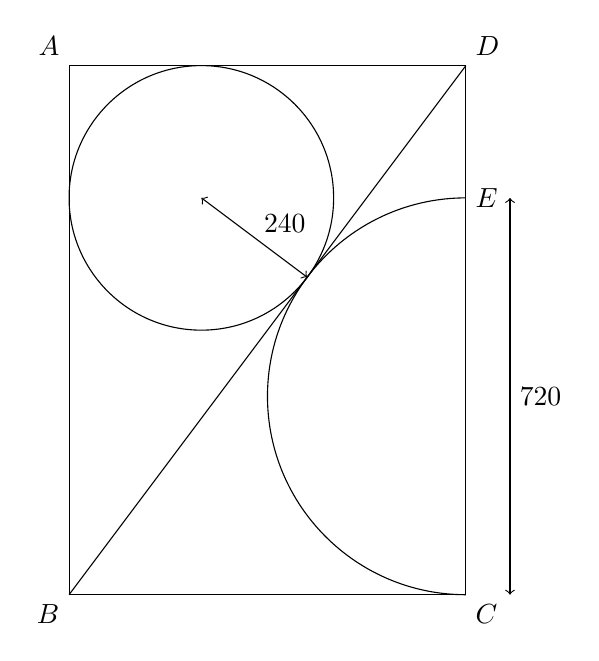
\begin{tikzpicture}[scale=0.7]
            \coordinate[label=above left:$A$] (A) at (0, 9.6);
            \coordinate[label=below left:$B$] (B) at (0, 0);
            \coordinate[label=below right:$C$] (C) at (7.2, 0);
            \coordinate[label=above right:$D$] (D) at (7.2, 9.6);
            \coordinate[label=right:$E$] (E) at (7.2, 7.2);

            \draw (A) -- (B) -- (C) -- (D) -- (A);
            \draw (B) -- (D);

            \draw (2.4, 7.2) circle[radius=2.4];
            \draw (7.2, 7.2) arc(90:270:3.6);

            \draw[<->] (2.4, 7.2) -- (4.32, 5.76);
            \draw[<->] (8, 0) -- (8, 7.2);

            \node[anchor=west] at (8, 3.6) {720};
            \node[anchor=south west] at (3.36, 6.4) {240};
        \end{tikzpicture}
    \end{center}
\end{question}
\begin{solution*}
    Let $AB = x$ and $AD = y$. Recall that $A = rs$, where $A$ is the area of a triangle, $r$ is the inradius of the triangle, and $s$ is the semiperimeter of the triangle. Applying this formula on $\triangle ABD$, we have \[\frac{xy}{2} = 240\bp{\frac{x + y + \sqrt{x^2 + y^2}}{2}} = 120\bp{x + y + \sqrt{x^2 + y^2}} \tag{1}.\] Let $F$ be the reflection of $B$ across $CD$. Applying this formula on $\triangle BDF$, we have \[2\bp{\frac{xy}{2}} = 360\bp{\frac{\sqrt{x^2 + y^2} + \sqrt{x^2 + y^2} + 2y}{2}} \implies \frac{xy}{2} = 180\bp{\sqrt{x^2 + y^2} + y} \tag{2}.\] Equating (1) and (2), we see that \[120\bp{x + y + \sqrt{x^2 + y^2}} = 180\bp{\sqrt{x^2 + y^2} + y} \implies y = \frac{3x}{4}.\] Substituting this back into (2), we have \[\frac12 \bs{x\bp{\frac{3x}{4}}} = 180\bs{\sqrt{x^2 + \bp{\frac{3x}{4}}^2} + \frac{3x}{4}} \implies x = 960.\] Thus, $y = 720$, whence the perimeter of $ABCD = 2(x + y) = 3360$ mm.
\end{solution*}